\chapter{Discrete-Time Markov Chains}
\label{ch:dtmc}

We now transition from continuous-time stochastic processes to their discrete-time counterparts. While physical systems evolve continuously, many models in fields like biology, economics, and computer science are more naturally described at discrete time steps. This leads us to the study of \textbf{Discrete-Time Markov Chains (DTMCs)}, which provide a powerful framework for modeling systems that transition between a set of discrete states over time.

\section{Fundamental Properties}

A DTMC is a stochastic process characterized by a discrete state space and the Markov property.

\begin{definitionblock}[Discrete-Time Markov Chain]
A stochastic process $\{X_t\}$, where time $t$ is an integer ($t \in \mathbb{N}_0$), is a \textbf{DTMC} if it satisfies:
\begin{enumerate}
    \item \textbf{Discrete State Space:} The process can only occupy states from a finite or countably infinite set $S = \{s_1, s_2, \ldots, s_N\}$.
    \item \textbf{Markov Property:} The future state of the system depends only on its present state, not on the sequence of events that preceded it. Mathematically, we can write:
    $$
    P\left(X_{t+1} = \sigma \mid X_t, X_{t-1}, \ldots, X_0\right) = P\left(X_{t+1} = \sigma \mid X_t\right)
    $$
\end{enumerate}
\end{definitionblock}

This "memoryless" property is the cornerstone of Markov chain theory. It allows us to describe the entire system's dynamics using only the probabilities of one-step transitions.

\begin{tipsblock}[Is it really important that $N$ is finite?]
    No; in physics, it is common to work with infinite-dimensional (countable or even uncountable) state spaces and infinite matrices without difficulty.
\end{tipsblock}

\subsubsection{The Evolution of the Probability Distribution}

Let $P_\sigma(t)$ be the probability that the system is in state $\sigma \in S$ at time $t$. To find the probability of being in state $\sigma$ at the next time step, $t+1$, we can sum over all possible states $\delta$ the system could have been in at time $t$. Using the law of total probability:
$$
P(X_{t+1} = \sigma) = \sum_{\delta \in S} P(X_{t+1} = \sigma \mid X_t = \delta) P(X_t = \delta)
$$
Let's introduce more concise notation. Let $\theta_{\delta\sigma}(t) = P(X_{t+1} = \sigma \mid X_t = \delta)$ be the \textbf{transition probability} from state $\delta$ to state $\sigma$ at time $t$. The evolution equation becomes:
$$
P_\sigma(t+1) = \sum_{\delta \in S} P_\delta(t) \theta_{\delta\sigma}(t)
$$
If we organize the state probabilities into a row vector $P(t) = [P_{s_1}(t), P_{s_2}(t), \ldots]$ and the transition probabilities into a matrix $\Theta(t)$, where $(\Theta)_{\delta\sigma} = \theta_{\delta\sigma}(t)$, we can write this system in a matrix form:
$$
P(t+1) = P(t) \Theta(t)
$$

\subsection{The Time-Homogeneous Case}

In many applications, the transition probabilities do not depend on time. Such a chain is called \textbf{time-homogeneous}. In this case, the transition matrix $\Theta$ is constant. The evolution of the probability distribution over multiple steps is then found by repeatedly applying the matrix:
\begin{align*}
    P(1) &= P(0)\Theta \\
    P(2) &= P(1)\Theta = P(0)\Theta^2 \\
    &\vdots \\
    P(t) &= P(0)\Theta^t
\end{align*}
The state of the system at any future time $t$ is completely determined by the initial probability distribution $P(0)$ and the $t$-th power of the transition matrix.

\begin{definitionblock}[Stochastic Matrix]
The transition matrix $\Theta$ of a time-homogeneous DTMC has two fundamental properties and is known as a \textbf{(row) stochastic matrix}:
\begin{enumerate}
    \item \textbf{Non-negativity:} All its elements are probabilities, so $0 \le \theta_{\delta\sigma} \le 1$.
    \item \textbf{Rows sum to one:} From any given state $\delta$, the system must transition to \textit{some} state in $S$. Therefore, the sum of probabilities of transitioning out of state $\delta$ must be 1.
    $$
    \sum_{\sigma \in S} \theta_{\delta\sigma} = 1 \quad \text{for all } \delta \in S
    $$
\end{enumerate}
\end{definitionblock}

A noteworthy consequence of the structure of the transition matrix $\Theta$ is that if $P(t)$ is a probability distribution, i.e.,
$$
\sum_{\sigma \in S} P_\sigma(t) = 1 \qquad \text{and} \qquad P_\sigma(t) \in [0,1]
$$
then $P(t+1) = P(t)\Theta$ is also a probability distribution:
$$
\sum_{\sigma \in S} P_\sigma(t+1) = 1 \qquad \text{and} \qquad P_\sigma(t+1) \in [0,1]
$$
This guarantees that the probability distribution remains valid at each time step. Let's see why:

\begin{itemize}
    \item \textbf{Preservation of normalization:} The sum of all probabilities at time $t+1$ is
    $$
    \sum_{\sigma \in S} P_\sigma(t+1) = \sum_{\sigma \in S} \sum_{\delta \in S} P_\delta(t)\theta_{\delta\sigma}(t) = \sum_{\delta \in S} P_\delta(t) \sum_{\sigma \in S} \theta_{\delta\sigma}(t)
    $$
    Since each row of the transition matrix sums to 1 (i.e., $\sum_{\sigma \in S} \theta_{\delta\sigma}(t) = 1$ for all $\delta$), this becomes:
    $$
    = \sum_{\delta \in S} P_\delta(t) \cdot 1 = \sum_{\delta \in S} P_\delta(t)
    $$
    So, if the probabilities sum to 1 at time $t$, they will also sum to 1 at time $t+1$.

    \item \textbf{Non-negativity:} Since $P_\delta(t) \geq 0$ and $\theta_{\delta\sigma}(t) \geq 0$, it follows that $P_\sigma(t+1) \geq 0$ for all $\sigma$.
\end{itemize}

\vspace{0.5em}

In summary, the evolution equation preserves both the normalization and non-negativity of the probability distribution at every step.

\subsubsection{Eigenvalues and Steady State}

The long-term (asymptotic) behavior of a discrete-time Markov chain (DTMC) is determined by the eigenvalues and eigenvectors of its transition matrix $\Theta$. 

\vspace{0.5em}

A key property of any stochastic (row-stochastic) matrix is that it always has at least one eigenvalue equal to $1$ (i.e., $\lambda=1$). All other eigenvalues $\lambda_i$ satisfy $|\lambda_i| \leq 1$; that is, their absolute values are less than or equal to $1$.

\vspace{0.5em}

The presence of the eigenvalue $\lambda=1$ ensures that there exists a special probability distribution, called the \textbf{stationary distribution} (or steady state), usually denoted by $\pi$. This stationary distribution has the property that, if the system starts in $\pi$, it remains in $\pi$ after each time step:

$$
\pi = \pi \Theta
$$

In other words, $\pi$ is a \textbf{left eigenvector} of $\Theta$ with eigenvalue $1$. If $\lambda=1$ is a simple eigenvalue (i.e., its geometric multiplicity is one, which is typically the case for ergodic Markov chains), then the stationary distribution is unique.

\begin{observationblock}[The Right Eigenvector]
The \textbf{right eigenvector} of $\Theta$ corresponding to $\lambda=1$ is the column vector of all ones: $\mathbf{v} = [1, 1, \ldots, 1]^\top$. This is a direct consequence of the fact that each row of $\Theta$ sums to $1$:

$$
(\Theta \mathbf{v})_i = \sum_j \theta_{ij} v_j = \sum_j \theta_{ij} \cdot 1 = \sum_j \theta_{ij} = 1 = (1 \cdot \mathbf{v})_i
$$

\end{observationblock}

\subsubsection{Alternative Formulation: Column Vector Evolution}

In some texts, the probability distribution (PD) is represented as a column vector rather than a row vector. In this formalism, the evolution equation is written as

$$
P(t+1) = W P(t)
$$

where

$$
P(t) = \begin{pmatrix} P_1(t) \\ \vdots \\ P_N(t) \end{pmatrix}
\qquad \text{and} \qquad
W = \Theta^\top
$$

Here, $W$ is the transpose of the original transition matrix $\Theta$. The matrix $W$ is also a (column-)stochastic matrix: each of its columns sums to $1$, i.e.,

$$
\sum_{R=1}^N W_{R,C}(t) = \sum_{R=1}^N \theta_{C,R}(t) = 1 \qquad \forall\, C.
$$

A fundamental property of $W$ is that the row vector $z = (1,\, \ldots,\, 1)$ is a left eigenvector of $W$ associated with the eigenvalue $\lambda = 1$:

$$
z W = z.
$$

\section{Asymptotic Behavior of the Probability Distribution}

We have established that the evolution of the probability distribution is given by
$$
P(t) = P(0)\Theta^t
$$
To analyze the long-term behavior, it is useful to diagonalize the transition matrix $\Theta$ (when possible):
$$
\Theta = H \, \mathrm{Diag}\{\lambda_1, \lambda_2, \ldots, \lambda_N\} H^{-1}
$$
where $\lambda_i$ are the eigenvalues of $\Theta$ and $H$ is the matrix of corresponding eigenvectors. In the vast majority of cases, $\Theta$ is diagonalizable; in the rare cases where it is not, a Jordan decomposition can be used. Applying this decomposition, the evolution can be written as:
$$
P(t) = P(0) H \, \mathrm{Diag}\{\lambda_1^t, \lambda_2^t, \ldots, \lambda_N^t\} H^{-1}
$$

To interpret this result, recall the following key properties of stochastic (Markov) matrices:
\begin{itemize}
    \item The transition matrix $\Theta$ always has an eigenvalue $\lambda_1 = 1$.
    \item All other eigenvalues satisfy $|\lambda_i| \leq 1$. 
    \item If $P(0)$ is a valid probability distribution, then $P(t)$ remains a probability distribution for all $t$.
\end{itemize}

\vspace{0.5em}

In the long-time limit ($t \to \infty$), all terms involving $|\lambda_i| < 1$ decay to zero, and only the contribution from $\lambda_1 = 1$ remains. This leads to the emergence of a stationary (steady-state) distribution, \emph{except in the case where there is an eigenvalue $\lambda = -1$}. In that case, the probability distribution function (PDF) becomes periodic, oscillating between two (or more) values.

For completeness, let us also consider the evolution in terms of the right action of the transition matrix (i.e., treating $P(t)$ as a column vector and using the transpose $\Theta^\top$):
$$
W = \Theta^\top
$$
The $t$-step evolution is then given by
$$
W^t = V \, \mathrm{Diag}\{\lambda_1^t, \ldots, \lambda_N^t\} V^{-1}
$$
where $V$ is the matrix of right eigenvectors of $\Theta$.

\vspace{0.5em}

\textbf{Stationary Distribution:} In the limit $t \to \infty$, the system approaches a stationary distribution $P_\infty$ that satisfies
$$
P_\infty = P_\infty \Theta
$$
That is, $P_\infty$ is a \textbf{left eigenvector} of $\Theta$ with eigenvalue $1$. If the eigenvalue $\lambda = 1$ is simple (i.e., has geometric multiplicity one), then the stationary distribution is unique.

The stationary distribution must also satisfy the normalization condition:
$$
\sum_{\sigma} (P_\infty)_\sigma = 1
$$

In summary, the asymptotic behavior of a discrete-time Markov chain is governed by the spectral properties of its transition matrix. The existence and uniqueness of the stationary distribution are guaranteed under mild conditions, and the system will converge to this distribution regardless of the initial state, provided the chain is ergodic and aperiodic.

\section{Simple DTMCs and Graphical Representation}

A DTMC is often visualized as a directed graph where nodes represent the states and weighted edges represent the transition probabilities. This graphical representation is invaluable for building intuition about the system's dynamics.

For a general two-state system, $S=\{0,1\}$, with a transition matrix:
$$
\Theta = \begin{pmatrix} \theta_{00} & \theta_{01} \\ \theta_{10} & \theta_{11} \end{pmatrix}
$$
the corresponding graph is:

\vspace{-0.5em}

\begin{center}
    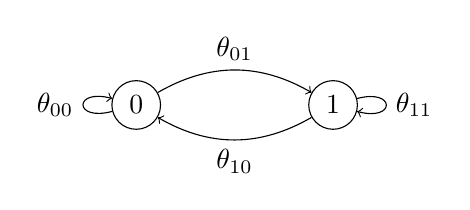
\begin{tikzpicture}
        \node[circle,draw] (s0) at (0, 0) {$0$};
        \node[circle,draw] (s1) at (2.5, 0) {$1$};
        \draw[->] (s0) to[loop left] node[left] {$\theta_{00}$} (s0);
        \draw[->] (s0) to[bend left=30] node[above] {$\theta_{01}$} (s1);
        \draw[->] (s1) to[bend left=30] node[below] {$\theta_{10}$} (s0);
        \draw[->] (s1) to[loop right] node[right] {$\theta_{11}$} (s1);
    \end{tikzpicture}
\end{center}

The evolution of the probability of being in state 0, $P_0(t)$, is given by:
$$
P_0(t+1) = \theta_{00} P_0(t) + \theta_{10} P_1(t)
$$
Since we only have two states, $P_1(t) = 1 - P_0(t)$. Substituting this we get:
$$
P_0(t+1) = \theta_{00} P_0(t) + \theta_{10} (1-P_0(t)) = (\theta_{00} - \theta_{10})P_0(t) + \theta_{10}
$$
The stationary probability, $P_0^{eq}$, is found by setting $P_0(t+1) = P_0(t) = P_0^{eq}$, which yields:
$$
P_0^{eq} = \frac{\theta_{10}}{1 - (\theta_{00} - \theta_{10})} = \frac{\theta_{10}}{(1-\theta_{00}) + \theta_{10}} = \frac{\theta_{10}}{\theta_{01} + \theta_{10}}
$$
We can now calculate the stationary probability of being in state 1:
$$
P_1^{eq} = 1 - P_0^{eq} = \frac{\theta_{01}}{\theta_{01} + \theta_{10}}
$$
This general result provides the long-term probability of finding the system in state 0, provided the system is ergodic. Let's now explore some specific cases.

\begin{exampleblock}[A Simple Absorbing Chain]
Consider a two-state Markov chain with states $S = \{0, 1\}$, where the transition probabilities are $\theta_{01} = 1$ and $\theta_{11} = 1$.

\vspace{-0.5em}

\begin{center}
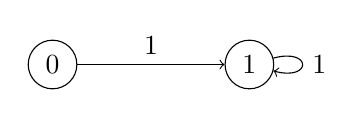
\begin{tikzpicture}
    \node[circle,draw] (s0) at (0, 0) {$0$};
    \node[circle,draw] (s1) at (2.5, 0) {$1$};
    \draw[->] (s0) to node[above] {$1$} (s1);
    \draw[->] (s1) to[loop right] node[right] {$1$} (s1);
\end{tikzpicture}
\end{center}

The transition matrix for this system is:

\vspace{-0.5em}

$$
\Theta = \begin{pmatrix} 0 & 1 \\ 0 & 1 \end{pmatrix}
$$
If the system starts in state 0 ($P(0) = [1,0]$), it moves to state 1 in one step and stays there permanently. If it starts in state 1, it remains there. Therefore, regardless of the initial state, the system will always end up in state 1. The stationary (limiting) distribution is:
$$
P(\infty) = [0, 1]
$$
State 1 is called \bfit{absorbing state} because, once entered, the probability of leaving it is zero.
\end{exampleblock}

\begin{exampleblock}[A Periodic Chain: The Flip-Flop]
Consider a system that \textbf{deterministically alternates} between two states, $S = \{0, 1\}$. In this Markov chain, the only possible transitions are from state 0 to state 1 and from state 1 to state 0, both with probability 1. That is, $\theta_{01} = 1$ and $\theta_{10} = 1$, while $\theta_{00} = \theta_{11} = 0$.

\begin{center}
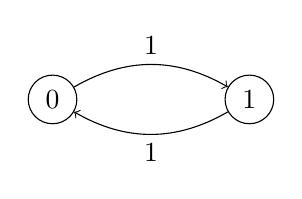
\begin{tikzpicture}
    \node[circle,draw] (s0) at (0, 0) {$0$};
    \node[circle,draw] (s1) at (2.5, 0) {$1$};
    \draw[->] (s0) to[bend left=30] node[above] {$1$} (s1);
    \draw[->] (s1) to[bend left=30] node[below] {$1$} (s0);
\end{tikzpicture}
\end{center}

The transition matrix for this system is:

$$
\Theta = \begin{pmatrix} 0 & 1 \\ 1 & 0 \end{pmatrix}
$$

Let $P_0(t)$ denote the probability of being in state 0 at time $t$. The evolution equation is:

$$
P_0(t+1) = \theta_{00} P_0(t) + \theta_{10} P_1(t) = 0 \cdot P_0(t) + 1 \cdot (1 - P_0(t)) = 1 - P_0(t)
$$

or, equivalently,

$$
P_0(t+1) = P_1(t) = 1 - P_0(t) 
$$

This is a simple linear recurrence relation. Its general solution is:

$$
P_0(t) = \left(P_0(0) - \frac{1}{2}\right)(-1)^t + \frac{1}{2}
$$

where $P_0(0)$ is the initial probability of being in state 0.

\vspace{0.5em}

The probability $P_0(t)$ alternates between two values, depending on whether $t$ is even or odd. The system never settles into a steady state; instead, it exhibits \textbf{periodic behavior} with period 2. This persistent oscillation is a direct consequence of the transition matrix $\Theta$ having eigenvalues $\lambda = 1$ and $\lambda = -1$.

The presence of an eigenvalue of $-1$ means that the system's state alternates in sign every time step, preventing convergence to a unique stationary distribution.
\end{exampleblock}

It is important to recognize that the discrete "time" variable $t$ in a Discrete-Time Markov Chain (DTMC) does not always correspond to physical time. While in some applications $t$ may indeed represent actual time steps (such as days, hours, or generations), in many contexts it serves as a convenient indexing parameter for the sequence of events or observations, regardless of whether these are temporally spaced.

For instance, in natural language processing, $t$ might index the position of a letter or word in a string of text, allowing a DTMC to model the probabilistic structure of language. In clinical studies, $t$ could denote the sequence number of a patient's follow-up visit, rather than a specific time interval. Similarly, in genetics, $t$ might represent generations in a population, or in queueing theory, the order of customer arrivals.

A particularly illustrative example is the discrete-time SIR (Susceptible-Infected-Recovered) model in epidemiology. Although infection and recovery are inherently continuous-time processes, modeling them in discrete time, such as updating the state of the system day by day, can provide a practical and insightful approximation. This approach enables the use of DTMCs to capture the essential dynamics of the system while simplifying analysis and computation.

\newpage

\section{Structural Properties of DTMCs}
We have so far informally used graphs to represent DTMCs, as they provide valuable insight into the internal structure and dynamics of the chain. We now give a formal definition:

\begin{definitionblock}[Support Graph of a DTMC]
Given a DTMC with state space $S$ and transition matrix $\Theta = (\theta_{ij})$, the \textbf{support graph} is the directed graph $G = (N, E)$ defined as follows:
\begin{itemize}
    \item The set of nodes is $N = S$ (the set of states).
    \item The set of directed edges is $E = \{ (i, j) \mid \theta_{ij} > 0 \}$; that is, there is an edge from $i$ to $j$ if and only if the transition probability from $i$ to $j$ is positive.
\end{itemize}
\end{definitionblock}

\subsubsection{Communicating Classes and Irreducibility}
The strongly connected components of the support graph correspond to the \textbf{communicating classes} of the DTMC. Two states, $i$ and $j$, are said to \textbf{communicate} (written $i \leftrightarrow j$) if it is possible to reach $j$ from $i$ and also to return from $j$ to $i$, each in a finite number of steps. This communication relation is an equivalence relation, partitioning the state space $S$ into disjoint communicating classes.

A Markov chain is called \textbf{irreducible} if there is only one communicating class; that is, every state can be reached from every other state. Such a chain is sometimes also called \textbf{ergodic}. If this is not the case, the chain is said to be \textbf{reducible}.

\begin{figure}[H]
    \centering
    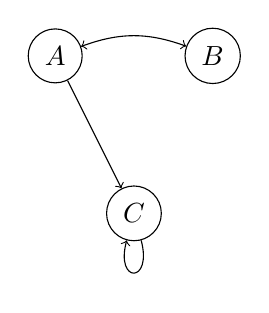
\begin{tikzpicture}
        % Class 1: A and B
        \node[circle,draw] (A) at (0, 0) {$A$};
        \node[circle,draw] (B) at (2, 0) {$B$};
        \draw[<->, bend left=20] (A) to (B);
        
        % Class 2: C
        \node[circle,draw] (C) at (1, -2) {$C$};
        \draw[->] (C) to[loop below] (C);

        % Transitions between classes
        \draw[->] (A) to (C);
    \end{tikzpicture}
    \caption{A reducible Markov chain with two communicating classes: $\{A, B\}$ and $\{C\}$.}
\end{figure}

\vspace{-1.5em}

\subsubsection{Recurrence and Transience}
A state $i$ is called \textbf{recurrent} if, starting from $i$, the probability of eventually returning to $i$ is 1. If this probability is less than 1, then $i$ is called \textbf{transient}.
\begin{itemize}
    \item In any finite Markov chain, at least one state must be recurrent.
    \item If $i$ is recurrent and communicates with $j$, then $j$ is also recurrent. So, recurrence is a property of the whole communicating class.
    \item If $i$ is transient, the expected number of visits to $i$ is finite; eventually, the process will leave $i$ and not return.
\end{itemize}
A recurrent state $i$ is called \textbf{positive recurrent} if the expected time to return to $i$ (starting from $i$) is finite. In finite Markov chains, all recurrent states are automatically positive recurrent.

\subsubsection{Periodicity}
A state $i$ has a \textbf{period} $d(i)$ if any return to $i$ must occur in a number of steps that is a multiple of $d(i)$, where $d(i)$ is the greatest common divisor of all possible return times to $i$. If $d(i) = 1$, the state is called \textbf{aperiodic}. Like recurrence, periodicity is a class property: all states in a communicating class share the same period. A DTMC is called aperiodic if all its states are aperiodic.

The "flip-flop" chain discussed earlier is a classic example of a periodic chain with period 2.

\newpage

\section{Absorbing States and Long-Term Behavior}

A special and important case in DTMC analysis is the presence of absorbing states.

\begin{definitionblock}[Absorbing State and Subgraph]
A state $s$ is an \textbf{absorbing state} if the probability of remaining in that state is 1, i.e., $\theta_{ss}=1$.

More generally, a communicating class $C$ is an \textbf{absorbing subgraph} if there are no transitions leading from any state in $C$ to any state outside of $C$.
\end{definitionblock}

In any DTMC with absorbing states, every non-absorbing state must be transient. This means the process will eventually leave the transient states and get "trapped" in one of the absorbing states or subgraphs forever. The long-term behavior of the system is therefore determined by which absorbing class it enters.

\begin{exampleblock}[The General Case with Multiple Absorbing States]
    The situation becomes more interesting when there are multiple absorbing states. Let's consider a system with three states, where states 1 and 2 are absorbing, and state 0 is transient. The corresponding graph is:
    \begin{center}
    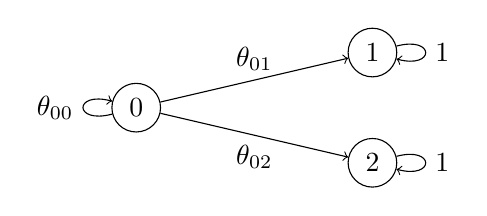
\begin{tikzpicture}
        \node[circle, draw] (s0) at (0,1) {0};
        \node[circle, draw] (s1) at (3,1.7) {1};
        \node[circle, draw] (s2) at (3,0.3) {2};
        \draw[->] (s0) to[loop left] node[left] {$\theta_{00}$} (s0);
        \draw[->] (s0) to node[above] {$\theta_{01}$} (s1);
        \draw[->] (s0) to node[below] {$\theta_{02}$} (s2);
        \draw[->] (s1) to[loop right] node[right] {$1$} (s1);
        \draw[->] (s2) to[loop right] node[right] {$1$} (s2);
    \end{tikzpicture}
    \end{center}
    The evolution equations for the probabilities are:
    $$
    \begin{array}{rl}
        P_0(t+1) &= \theta_{00}P_0(t) \\
        P_1(t+1) &= \theta_{01}P_0(t) + P_1(t) \\
        P_2(t+1) &= \theta_{02}P_0(t) + P_2(t)
    \end{array}
    $$
    with the constraint that $\theta_{00} + \theta_{01} + \theta_{02} = 1$. The transition matrix for this system is:
    \small
    $$
    \Theta = \begin{pmatrix}
    \theta_{00} & \theta_{01} & \theta_{02} \\
    0 & 1 & 0 \\
    0 & 0 & 1
    \end{pmatrix}
    $$
    \normalsize
    From the first equation, we see that $P_0(t) = P_0(0)(\theta_{00})^t$. Since $\theta_{00} < 1$ (otherwise the other states would be unreachable), $P_0(t) \to 0$ as $t \to \infty$. This confirms that state 0 is transient.
    
    The probability mass that leaves state 0 at each step is distributed between states 1 and 2. To find the final distribution, we can sum the increments to $P_1(t)$ and $P_2(t)$ over all time:
    $$
    P_1(\infty) = P_1(0) + \sum_{t=0}^{\infty} \theta_{01} P_0(t) = P_1(0) + \theta_{01} P_0(0) \sum_{t=0}^{\infty} (\theta_{00})^t
    $$
    Using the formula for a geometric series, $\sum_{t=0}^{\infty} r^t = 1/(1-r)$, we get:
    $$
    P_1(\infty) = P_1(0) + P_0(0) \frac{\theta_{01}}{1-\theta_{00}}
    $$

    \vspace{-0.7em}

    Similarly for state 2:

    \vspace{-0.7em}

    $$
    P_2(\infty) = P_2(0) + P_0(0) \frac{\theta_{02}}{1-\theta_{00}}
    $$
    The final distribution is therefore $P(\infty) = [0, P_1(\infty), P_2(\infty)]$ and it depends on the initial distribution $P(0)$ and the transition probabilities out of the transient state. The eigenvalue $\lambda=1$ has a geometric multiplicity of 2, corresponding to the two absorbing states.
    \end{exampleblock}


\subsection{Probability of Absorption}
Let $A$ be an absorbing subset of states in a DTMC. The \textbf{probability of absorption}, $h_i^A$, is the probability that the process will eventually enter the set $A$, given that it starts in state $i \notin A$.
$$
h_i^A = P(\text{the process eventually enters } A \mid X_0 = i)
$$
By conditioning on the first step, we can establish a system of linear equations for these probabilities. From state $i$, the process transitions to some state $j$ with probability $\theta_{ij}$. From there, the probability of being absorbed into $A$ is $h_j^A$. Therefore:
$$
h_i^A = \sum_{j \in S} \theta_{ij} h_j^A
$$
This system must be solved with the boundary conditions:
\begin{itemize}
    \item $h_i^A = 1$ if $i \in A$ (already absorbed).
    \item $h_i^A = 0$ if state $i$ cannot reach any state in $A$.
\end{itemize}
Solving this system gives the absorption probabilities for all transient states.

\subsection{Permanence Time}
The \textbf{permanence time} is the number of consecutive steps a process stays in a given state before leaving it. Consider state $s \in S$, with the process starting at $X_0 = s$. Let $T$ be the random variable for the number of steps the process remains in $s$ before moving to any other state. The event $T = t$ means the process stays in $s$ for $t$ steps, then leaves to some $y \neq s$ at step $t+1$. The probability is:
$$
P(T = t) = P(X_{t+1} \neq s, X_t=s, \ldots, X_1=s \mid X_0=s)
$$
Due to the Markov property, we can factorize this conditional probability:
$$
P(T=t) = P(X_1=s \mid X_0=s) \times \ldots \times P(X_t=s \mid X_{t-1}=s) \times P(X_{t+1} \neq s \mid X_t=s) = (\theta_{ss})^t \times \sum_{y \neq s} \theta_{sy}
$$

\vspace{-0.5em}

Since the rows of the transition matrix must sum to one, it follows that the probability of leaving state $s$ is $\sum_{y \neq s} \theta_{sy} = 1 - \theta_{ss}$. Therefore, the probability distribution of the permanence time is:
$$
P(T = t) = (\theta_{ss})^t (1-\theta_{ss})
$$
This is the probability mass function of a \textbf{geometric distribution}. It is straightforward to verify that this is a valid probability distribution by summing over all possible times $t \ge 0$:
$$
\sum_{t=0}^{\infty} P(T=t) = (1-\theta_{ss}) \sum_{t=0}^{\infty} (\theta_{ss})^t = (1-\theta_{ss}) \left( \frac{1}{1-\theta_{ss}} \right) = 1
$$
The \textbf{mean permanence time} in state $s$ is the expected value of this geometric distribution:
$$
\langle T \rangle = \frac{\theta_{ss}}{1-\theta_{ss}}
$$
Alternatively, if we start from state $s$, the mean permanence time is:
$$
\langle T \rangle = \frac{1}{1-\theta_{ss}}
$$
The closer $\theta_{ss}$ is to 1, the longer the process is expected to remain in that state before transitioning. In the limit of an absorbing state ($\theta_{ss}=1$), the mean permanence time is infinite.

\section{Ergodicity}

A DTMC is said to be \textbf{ergodic} if it is both irreducible (all states communicate) and aperiodic (no deterministic cycles). More formally, a chain is ergodic if for any two states $i,j$, there exists an integer $n_0$ such that the probability of transitioning from $i$ to $j$ in $n$ steps is positive for all $n \ge n_0$:
$$
(\Theta^n)_{ij} > 0 \quad \text{for all } n \ge n_0
$$

Ergodicity is a crucial property because it guarantees a simple and predictable long-term behavior.

\subsection{Properties of Ergodic Chains}
If a DTMC is ergodic, it has several important properties:
\begin{enumerate}
    \item \textbf{Unique Stationary Distribution:} There exists a unique equilibrium probability distribution, $\pi$, which is independent of the initial conditions.
    
    \item \textbf{Convergence to Stationary Distribution:} For any initial distribution $P(0)$, the probability distribution at time $t$ will converge to this unique stationary distribution $\pi$ as $t \to \infty$.
    $$
    \lim_{t \to \infty} P(t) = \pi
    $$
    Furthermore, for sufficiently large $t$, this convergence is typically exponential, meaning $P(t) \approx \pi + O(e^{-qt})$ for some rate $q > 0$.
    
    \item \textbf{Equivalence of Time and Ensemble Averages:} This is the most profound consequence of ergodicity. It states that the long-term time average of any function of the state is equal to the ensemble average (the expected value) of that function under the stationary distribution.
    
    For a function $A(x(t))$, the well-known law of large numbers for ergodic processes states:
    $$
    \underbrace{\lim_{T \to \infty} \frac{1}{T} \sum_{t=1}^T A(x(t))}_{\text{Time Average}} = \underbrace{\sum_{s \in S} A(s)\pi_s}_{\text{Ensemble Average}}
    $$
\end{enumerate}

\subsection{Inferring the Stationary Distribution from Data}
The property of ergodicity provides a powerful practical tool: we can infer the stationary distribution by analyzing a single, sufficiently long time series from the process.

Let's define a specific function $A(s) = \delta(s-r)$, which is 1 if the state $s$ is our target state $r$, and 0 otherwise. The ensemble average is simply $\sum_s \delta(s-r)\pi_s = \pi_r$. The time average becomes the long-term frequency of visits to state $r$:
$$
\lim_{T \to \infty} \frac{1}{T} \sum_{t=1}^T \delta(x(t)-r) = \lim_{T \to \infty} \frac{\text{Number of visits to state } r}{T}
$$
The ergodic property guarantees that these two are equal:
$$
\pi_r = \lim_{T \to \infty} \frac{\text{Number of visits to state } r}{\text{Total number of observations}}
$$
This means we can estimate the stationary probability of a state by simply measuring how often it occurs in a long simulation.

\subsection{The Kac Lemma: Return Times}
We have already encountered the \textbf{Kac Lemma} in \cref{sec:kac}, where it was discussed in the context of continuous-time Markov processes. The result applies equally to DTMCs: it provides a direct link between the stationary probability of a state and the expected time to return to it.

Let $T_s$ be the random variable representing the \textbf{first return time} to state $s$, given that the process starts in state $s$. The Kac Lemma states that the expected value of this return time is the reciprocal of the stationary probability of that state:
$$
\mathbb{E}[T_s] = \frac{1}{\pi_s}
$$
This relationship is highly intuitive:
\begin{itemize}
    \item If a state $s$ is rarely visited, its stationary probability $\pi_s$ is small. Consequently, the mean return time $\mathbb{E}[T_s]$ will be very long.
    \item If a state $s$ is frequently visited, its probability $\pi_s$ is close to one. The mean return time will be minimal, i.e., slightly larger than one.
\end{itemize}

\section{Kolmogorov Equations}

...

% \subsubsection{Apparent Paradox}

% \begin{exampleblock}[The Gambler's Ruin]
%     A classic example of a system with multiple absorbing states is the \textbf{Gambler's Ruin}. A gambler starts with an initial capital of $i$ dollars and repeatedly plays a game, winning \$1 with probability $p$ and losing \$1 with probability $q=1-p$. The game ends when the gambler is either ruined (capital reaches \$0) or wins a target amount of $N$ dollars.
    
%     The states are the gambler's capital, $S = \{0, 1, \ldots, N\}$. The states $0$ and $N$ are absorbing states. The transition matrix for $N=4$ is:
%     $$
%     \Theta = \begin{pmatrix}
%     1 & 0 & 0 & 0 & 0 \\
%     q & 0 & p & 0 & 0 \\
%     0 & q & 0 & p & 0 \\
%     0 & 0 & q & 0 & p \\
%     0 & 0 & 0 & 0 & 1
%     \end{pmatrix}
%     $$
%     The system must eventually end up in state 0 or N. The probability of being ruined (reaching state 0) starting from state $i$ is a classic result in probability theory.
% \end{exampleblock}